\chapter{Display}

In diesem Kapitel gehen wir auf das Display ein, das im \textbf{Spiegel AI} Projekt verwendet wird. Wir beschreiben die Spezifikationen, die Installation und die Anpassungen, die vorgenommen wurden.

\section{Spezifikationen}
Beschreiben Sie die technischen Spezifikationen des Displays.

\section{Installation}
Erläutern Sie den Prozess der Installation des Displays.

\section{Anpassungen}
Beschreiben Sie etwaige Anpassungen oder Modifikationen am Display.

\subsection{eventuell HTMl seite und Aufbau oder in Installation}
\subsection{Widget 1}
\subsection{Widget 2}
\subsection{Widget 3}
\subsection{Widget 4}
\subsection{Uhr Widget}
Erarbeitet von: Marcel Wagner \\ \\
\noindent
Die Implementierung des Uhrzeit Widgets für den Smart Mirror ist ein wichtiger Schritt zur Verbesserung der Funktionalität und Benutzerfreundlichkeit des Geräts. Ziel dieses Widgets ist es, die aktuelle Uhrzeit exakt und zuverlässig anzuzeigen. Wobei die Anzeige in Echtzeit aktualisiert werden muss, um stets die genaue Uhrzeit widerzuspiegeln.\\ \\
Die Implementierung dieses Widgets basierte auf der Nutzung von JavaScript zur Echtzeitaktualisierung der Uhrzeit und HTML zur Einbettung des Widgets in die Benutzeroberfläche des Smart Mirrors. Desweiteren wurde CSS benutzt um das Widget zu formatieren. Die JavaScript Funktion sorgt dafür, dass die Uhrzeit jede Sekunde aktualisiert wird, während das HTML Dokument die Struktur definiert. Abschließend definiert die CSS Datei das Styling des Widgets. \\ \\
\noindent
Während der Entwicklung des Widgets traten mehrere Herausforderungen auf. Eine der größten Herausforderungen bestand darin, sicherzustellen, dass die Uhrzeit in Echtzeit und ohne Verzögerung aktualisiert wird. Dies war besonders wichtig, um die Genauigkeit der angezeigten Zeit zu gewährleisten. Die Verwendung der 'setTimeout' Funktion in JavaScript ermöglicht eine wiederholte Ausführung der Aktualisierungsfunktion in einem festgelegten Intervall von einer Sekunde, wodurch eine kontinuierliche und genaue Aktualisierung der Uhrzeit sichergestellt wurde.
Eine weitere Herausforderung war die exakte Zeitanzeige, insbesondere hierbei ist wichtig die Erwähnung der Formatierung der Uhrzeit, um sicherzustellen, dass Stunden, Minuten und Sekunden stets zweistellig angezeigt werden. Durch die Verwendung der 'padStart' Methode konnten die Zahlen auf eine konstante Länge von zwei Stellen gebracht werden, indem bei Bedarf führende Nullen hinzugefügt werden. Dies gewährleistete eine konsistente und gut lesbare Anzeige.\\ \\
\noindent
Die Implementierung des Uhrzeit Widgets verlief erfolgreich und erfüllt die gestellten Anforderungen. Die Uhrzeit wird zuverlässig und exakt in Echtzeit angezeigt. Das Widget integriert sich nahtlos in die Benutzeroberfläche des Smart Mirrors und bietet eine klare und gut lesbare Darstellung der aktuellen Uhrzeit.
Insgesamt stellt das Uhrzeit Widget eine wesentliche Funktionalität des Smart Mirrors dar. Der nachfolgenden Abbildung 1 kann das Implementierte Uhrzeit Widget auf der HTML Seite entnommen werden.

\begin{figure}[h]
    \centering
    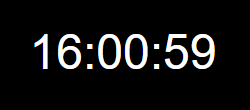
\includegraphics[width=0.4\textwidth]{pictures/time_widget.png}
  \captionsetup{justification=centering, labelformat=simple, singlelinecheck=false}
    \caption[Uhrzeit Widget]{Uhrzeit Widget\\ Quelle: eigene Darstellung}
\end{figure}

\subsection{Verkehrsinformation}
Erarbeitet von: Marcel Wagner \\ \\
\noindent
Die Implementierung des Stau-Widgets auf dem Smart Mirror stellt einen wichtigen Schritt dar, um den Nutzern eine umfassende und zuverlässige Quelle für aktuelle Verkehrsinformationen zur Verfügung zu stellen. Das Widget wurde speziell entwickelt, um eine Echtzeitübersicht über die Verkehrslage in Regensburg zu bieten, was insbesondere für Pendler und Reisende von großem Nutzen ist. Durch die Verwendung von JavaScript wurde eine nahtlose Integration mit der OpenStreetMap Overpass API realisiert, die als zuverlässige Datenquelle für Verkehrsdaten dient. \\ \\
\noindent
Die Strategie hinter der Implementierung war zweigleisig: Zum einen wurde eine sofortige Aktualisierung der Verkehrsinformationen beim Laden der Seite implementiert, um den Nutzern bei jedem Besuch des Smart Mirrors die aktuellsten Daten bereitzustellen. Zum anderen erfolgt eine regelmäßige automatische Aktualisierung alle fünf Minuten, um sicherzustellen, dass die angezeigten Informationen kontinuierlich aktuell gehalten werden. Dieser Ansatz gewährleistet eine hohe Aktualität und Relevanz der bereitgestellten Verkehrsinformationen. \\ \\
\noindent
Während der Entwicklung wurden mehrere Herausforderungen gemeistert, darunter die robuste Fehlerbehandlung, um sicherzustellen, dass Netzwerkprobleme oder API Ausfälle die Funktionalität des Widgets nicht beeinträchtigen. Ein besonderes Augenmerk lag auf der Gewährleistung einer stabilen und zuverlässigen Datenaktualisierung, die für eine nahtlose Benutzererfahrung entscheidend ist. \\ \\
\noindent
Das Verkehrs Widget präsentiert die Verkehrslage in einer klaren und intuitiven Benutzeroberfläche. Es informiert die Nutzer klar verständlich darüber, ob derzeit ein Stau vorliegt oder nicht, und bietet gegebenenfalls zusätzliche Informationen über Verkehrshindernisse oder Verkehrswarnungen. Diese klare visuelle Darstellung hilft den Nutzern, schnell zu erfassen, wie die aktuelle Verkehrssituation ihre geplante Route beeinflussen ist. \\ \\
\noindent
Insgesamt trägt das Verkehrs Widget erheblich zur Funktionalität und Benutzerfreundlichkeit des Smart Mirrors bei. Es bietet eine unverzichtbare Informationsquelle für die tägliche Routenplanung und unterstützt die Nutzer dabei, ihre Fahrtzeiten effizient zu optimieren. Das Implementierte Verkehrsinformationen Widget kann der nachfolgenden Abbildung entnommen werden. Diese Abbildung zeigt den Fall, dass aktuell gerade kein Stau  in den Straßen von Regensburg sind.

\begin{figure}[h]
    \centering
    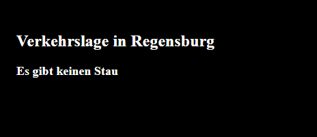
\includegraphics[width=0.4\textwidth]{pictures/traffic_widget.png}
  \captionsetup{justification=centering, labelformat=simple, singlelinecheck=false}
    \caption[Verkehrsinformations Widget]{Verkehrsinformations Widget\\ Quelle: eigene Darstellung}
\end{figure}

\subsection{Schlagzeilen}
Erarbeitet von: Marcel Wagner \\ \\
\noindent
Die Implementierung des Nachrichten Widgets für den Smart Mirror stellt einen wichtigen Schritt dar, um den Nutzern eine aktuelle und relevante Informationsquelle direkt auf seinem Smart Mirror zur Verfügung zu stellen. Das Widget wurde in JavaScript entwickelt und verwendet die 'RSS2JSON-API', um die neuesten Nachrichtenartikel eines ausgewählten RSS Feeds abzurufen und auf dem Smart Mirror anzuzeigen. Dies ermöglicht eine dynamische und automatische Aktualisierung der Nachrichteninhalte, sobald der Nutzer den Spiegel nutzt. \\ \\
\noindent
Ein zentrales Element der Implementierung ist die Verwendung des 'DOMContentLoaded' Events, das sicherstellt, dass das Widget erst aktiv wird, nachdem die gesamte Seite vollständig geladen ist. Dadurch wird sichergestellt, dass alle notwendigen Ressourcen und Elemente bereitstehen, bevor die Datenabfrage und die Darstellung der Nachrichten beginnen. \\ \\
\noindent
Die Funktionalität des Widgets umfasst die Asynchronität der Datenabfrage über die Fetch API, die die RSS Feeds von Nachrichtenquellen in ein JSON Format umwandelt, das vom JavaScript Code weiterverarbeitet werden kann. Dies ermöglicht eine schnelle und effiziente Bereitstellung der neuesten Nachrichteninhalte direkt auf dem Smart Mirror, ohne dass der Nutzer zusätzliche Schritte unternehmen muss, um sich auf dem Laufenden zu halten. \\ \\
\noindent
Eine besondere Herausforderung während der Implementierung war die unterschiedliche Verfügbarkeit von RSS Feeds bei verschiedenen Nachrichtenseiten. Viele führende Nachrichtenagenturen und Zeitungen bieten zwar RSS Feeds an, einige jedoch nicht oder beschränken den Zugang zu ihren Inhalten über diese Schnittstelle. Dies erforderte eine sorgfältige Auswahl geeigneter RSS Feeds, die eine kontinuierliche und zuverlässige Datenversorgung gewährleisten konnten. Die Ausgegeben Nachrichten dieses Widget entspannen der Frankfurter Allgemeinen Zeitung \\ \\
\noindent
Um die Benutzerfreundlichkeit zu maximieren, wurde die Benutzeroberfläche des Widgets bewusst einfach und intuitiv gestaltet. Die angezeigten Nachrichten werden in einer geordneten Liste präsentiert. \\ \\
\noindent
Zusammenfassend bietet das Nachrichten Widget einen bedeutenden Mehrwert für den Smart Mirror, indem es den Nutzern eine einfache und effektive Möglichkeit bietet, sich über aktuelle Ereignisse zu informieren. Die Implementierung war erfolgreich in Bezug auf die gesetzten Ziele. Der Nachfolgenden Abbildung kann das implementierte Widget auf dem Smart Mirror entnommen werden.

\begin{figure}[h]
    \centering
    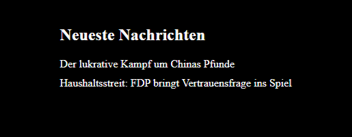
\includegraphics[width=0.4\textwidth]{pictures/news_widget.png}
  \captionsetup{justification=centering, labelformat=simple, singlelinecheck=false}
    \caption[News Widget]{News Widget\\ Quelle: eigene Darstellung}
\end{figure}

\subsection{Tankstellen}
Erarbeitet von: Marcel Wagner \\ \\
\noindent
Die Implementierung des Tankstellen Widgets für den Smart Mirror verfolgt das Ziel, den Nutzern eine praktische und zeitnahe Information über den günstigsten Kraftstoffpreise einer Tankstelle in der Nähe zu bieten. Diese Funktionalität wurde durch die Integration von JavaScript und die Nutzung der Tankerkoenig API realisiert, die speziell auf die Abfrage von Tankstellenpreisen und Tankstelleninformationen ausgerichtet ist. \\ \\
\noindent
Zu Beginn des Implementierungsprozesses wird der 'DOMContentLoaded' Eventlistener verwendet, um sicherzustellen, dass sämtliche Inhalte der Webseite geladen sind, bevor die Datenabfrage gestartet wird. Dies gewährleistet eine stabile und zuverlässige Performance des Widgets auf dem Smart Mirror. Die API Anfrage erfolgt unter Verwendung eines spezifischen API Schlüssels, der die Authentifizierung gegenüber der Tankerkoenig API ermöglicht. Der Standortbezug erfolgt für die Stadt Regensburg mit definierten geografischen Koordinaten und einem Suchradius von 5 Kilometern, um die Tankstellen in unmittelbarer Umgebung zu erfassen. \\ \\
\noindent
Die Datenabfrage wird asynchron durchgeführt, um eine reibungslose Interaktion mit der API zu gewährleisten. Nachdem die Daten abgerufen wurden, erfolgt eine Überprüfung auf erfolgreiche Antwort und die Verfügbarkeit von Tankstelleninformationen. Falls die API Daten erfolgreich zurückgegeben werden und Tankstelleninformationen vorhanden sind, wird die günstigste Tankstelle ermittelt. Dies geschieht durch einen Vergleich der Kraftstoffpreise der abgerufenen Tankstellen, wobei die preisgünstigste Option ausgewählt und deren Informationen weiterverarbeitet werden. \\ \\
\noindent
Ein zentraler Aspekt der Implementierung ist die robuste Fehlerbehandlung, die sicherstellt, dass der Nutzer bei Problemen wie Netzwerkfehlern oder unerwarteten API Antworten angemessen informiert wird.  \\ \\
\noindent
Die Darstellung der Tankstelleninformationen auf dem Smart Mirror erfolgt in einer klar strukturierten Form. Dies umfasst den Namen der Tankstelle, die vollständige Adresse inklusive Straße, Hausnummer, Postleitzahl und Ort sowie den aktuellen Preis pro Liter Kraftstoff. Diese Informationen sind leicht zugänglich und ermöglichen es dem Nutzer, schnell die wichtigsten Details zu erfassen und eine informierte Entscheidung zu treffen. \\ \\
\noindent
Die Implementierung des Tankstellen Widgets erweitert somit die Funktionalität des Smart Mirrors erheblich, indem sie eine praktische Lösung für die Überwachung und Optimierung der Kraftstoffkosten bietet.

\begin{figure}[h]
    \centering
    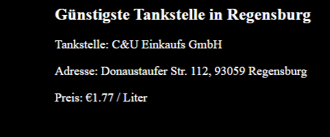
\includegraphics[width=0.4\textwidth]{pictures/gasstation_widget.png}
  \captionsetup{justification=centering, labelformat=simple, singlelinecheck=false}
    \caption[Tankstellen Widget]{Tankstellen Widget\\ Quelle: eigene Darstellung}
\end{figure}

\subsection{Test Verfahren}
Erarbeitet von: Leon Kranner und Marcel Wagner \\ \\
\noindent
Für die implementierten Widgets auf dem Smart Mirror wurden umfangreiche Testverfahren angewendet, die sowohl die Funktionalität als auch die Benutzererfahrung der einzelnen Widgets sicherstellen sollen. Diese unterschiedlichen Testverfahren werden nun im Folgenden genauer beschrieben. \\ \\
\noindent
\textbf{Funktionalitätstests:} Dieser Test konzentrierten sich auf die grundlegenden Aufgaben jedes Widgets. Das Uhrzeitwidget wurde auf seine Fähigkeit getestet, die aktuelle Uhrzeit präzise anzuzeigen. Außerdem wurde sichergestellt, dass die Darstellung formatiert und korrekt aktualisiert wird. Beim News Widget lag der Fokus auf der korrekten Abrufung und Darstellung aktueller Nachrichten, wobei sichergestellt wurde, dass die Informationen stets aktuell und relevant sind. Das Tankstellenwidget durchlief API Integrationstests, um sicherzustellen, dass die Kraftstoffpreise korrekt von der Tankerkoenig API abgerufen und in einem klaren Format angezeigt werden. Das Verkehrsinformations Widget wurde auf seine Fähigkeit geprüft, Verkehrsinformationen zeitnah abzurufen und zuverlässig darzustellen, um Nutzer vor aktuellen Verkehrsbehinderungen zu warnen. \\ \\
\noindent
\textbf{Benutzererfahrungstests:} Diese waren entscheidend, um sicherzustellen, dass die Widgets intuitiv sind. Hierbei halfen Usability Tests, diese bewerteten die Widgets auf Benutzerfreundlichkeit der Benutzeroberfläche. Dabei wurde besonders darauf geachtet, dass die Widgets übersichtlich gestaltet sind und Nutzer schnell die benötigten Informationen finden können. \\ \\
\noindent
\textbf{Performance- und Lasttests:} Diese Testverfahren waren ebenfalls Teil der Teststrategie, um sicherzustellen, dass die Widgets unter verschiedenen Bedingungen effizient arbeiten. Ladezeittests wurden durchgeführt, um sicherzustellen, dass die Widgets schnell genug reagieren und Daten effizient verarbeiten. Skalierbarkeitstests wurden genutzt, um sicherzustellen, dass die Widgets auch bei erhöhtem Datenverkehr stabil bleiben und keine übermäßigen Ressourcen verbrauchen, was besonders wichtig für die Langzeitnutzung ist. \\ \\
\noindent
\textbf{Integrationstest:} Dabei wurden Kompatibilitätstests durchgeführt, um sicherzustellen, dass die Widgets reibungslos mit anderen Komponenten des Smart Mirrors interagieren. Systemtests prüften die Gesamtfunktionalität des Smart Mirrors unter verschiedenen Betriebsbedingungen, um sicherzustellen, dass alle Widgets harmonisch zusammenarbeiten und die Gesamtleistung des Systems nicht beeinträchtigen werden. \\ \\
\noindent
Diese umfassenden Testverfahren stellen sicher, dass die implementierten Widgets nicht nur funktional sind, sondern auch eine qualitativ hochwertige Benutzererfahrung bieten und unter allen Bedingungen zuverlässig arbeiten.



